\lstset{style=phpstyle}

\section{Обзор предметной области}
\label{sec:domain}

\subsection{Системы учета времени}
\label{sub:domain:time_managament_systems}
Учет времени подразумевает использование ежедневников, планнеров, составление списков дел, но не ограничивается ими. Под системой мы понимаем целостную структуру взаимосвязанных деталей, где всё вышеперечисленное является лишь элементом. В целом же система управления временем – это специальная методика, зачастую с собственным инструментарием, а также рекомендациями и советами по эффективной организации своей деятельности. Её задача – не просто напомнить о каком-либо занятии или встрече, распланировать день (месяц, год), но и показать, как это сделать эффективно, чтобы не только завершить работу в срок, но и достичь большего. В классическом понимании системы учета времени и заложена суть: она помогает человеку и планировать занятость, и гибко управлять временем, затрачиваемым на разные нужды.

Сегодня существует около десятка наиболее известных систем управления временем и множество вариаций, основанных на личном опыте их применения. На форумах и в блогах можно найти достаточное количество примеров собственных систем, где авторы объединяют элементы нескольких методик, привнося новшества, или трактуя их под свою сферу занятости. В этом, в частности, заключается одна из главных полезностей: возможность «настроить» план «под себя», изменить, полностью отбросить или позаимствовать из других техник отдельные инструкции и детали. Благодаря этому, системы управления временем может применять каждый: инженер и журналист, офисный сотрудник и фрилансер, тот, кто распределяет рабочее время и тот, кто планирует отдых. Каждая из них имеет свои преимущества, поэтому рассмотрим несколько наиболее известных.


\subsection{Пирамида Франклина}

\label{page:domain:piramida_franklina}
\begin{figure}
\centering
  
\includegraphics[scale=0.85]{images/franklin_piramida.jpg}
  \caption{ Пирамида Франклина }
  \label{fig:domain:franklin}
\end{figure}


Структура системы представляется как пирамида, где каждый элемент зависит от предыдущего это целостная система постановки и реализации целей. Ее главной особенностью является направленность на результат и планомерное движение от общего к частному. Весь жизненный распорядок, таким образом, подчинен достижению главных жизненных целей. Система Франклина имеет следующую структуру: жизненные ценности, глобальная цель, генеральный план, долгосрочный план, краткосрочный план, план на день. 


1. Жизненные ценности – это базовые глобальные ценности. Это ответ на вопросы: «Ради чего я живу?», «Что для меня является самым важным в жизни?». Очень важно искренне ответить для себя на эти вопросы и не ошибиться при их определении. Кто-то находит смысл жизни в признании, во власти, кто-то в семье, для кого-то важнее всего обеспеченная жизнь и деньги, для других самосовершенствование и альтруизм и т.д. Если речь идет об организации, то «жизненные цели» – это ее миссия, глобальное предназначение, смысл существования. Например, миссия компании «Отис» (производители лифтов и эскалаторов) звучит так: «Мы помогаем людям перемещаться в пространстве». Миссия нефтяной компании – «Мы обеспечиваем энергией». 

2. Глобальная цель ставится на основании заявленных жизненных ценностей. Это «большая» цель, максимально желаемая. Например, спортсмен-марафонец, определивший, что для него самое важное – слава и известность, признание мирового Олимпа, решает стать чемпионом мира. 

3. Генеральный план – это большой и общий план по достижению глобальной цели. Например, для того чтобы стать олимпийским чемпионом, нужно иметь хорошее здоровье и физическую форму, физкультурное образование, отличного тренера, получить звание мастера спорта, победить на соревнованиях области/города/страны/Европы. 

4. Долгосрочный план – это план на несколько лет, с указанием конкретных целей и сроков. Для спортсмена важно участвовать в соревнованиях Восточной Европы и победить там. Для этого ему нужно, чтобы показатели его скорости пробега были больше, чем у прошлого чемпиона. Необходимо сформулировать цель следующим образом: «К 2011 году я должен пробегать 42 км за 2 часа – так я завоюю титул чемпиона Восточной Европы и буду приглашен на чемпионат Мира». 

5. Краткосрочный план – план на срок от нескольких недель до нескольких месяцев. Исходя из долгосрочного плана, важно определить, что можно сделать в течение ближайших нескольких недель и месяцев для достижения цели. Так, для нашего спортсмена – это увеличить количество тренировок, повысить выносливость организма, опробовать новую систему подготовки. 

6. План на день. Задачи из плана на неделю разбиваются на более мелкие, например, задача увеличить выносливость выглядит как: пойти в спортзал, заниматься на беговом тренажере 3 часа, пробежать 5 км за 20 мин, замерить пульс, записать результаты в дневник.

\subsection{Матрица Эйзенхауэра}
Матрица Эйзенхауэра (матрица приоритетов) – один из самых известных инструментов для управления своим временем. Ее придумал Дуайт Эйзенхауэр, 34-й президент США.

Поэтому Эйзенхауэр начал испытывать разные инструменты учета времени. Он хотел  найти нечто самое эффективное. Но так и не нашел такого, чтобы его удовлетворило. Поэтому, в конце концов, он создал собственный инструмент, который в последствии получил его имя.

Матрица Эйзенхауэра используется для планирования на небольшой срок (один или несколько дней). Это эффективный метод обработки тех списков дел, что человек планирует сделать за этот срок. Как правило, люди составляют столь длинные списки, что все дела из них априори невозможно переделать.

Представляет собой четыре квадранта, основанием которых служат две оси — это ось важности (по вертикали) и ось срочности (по горизонтали). В итоге получается, что каждый квадрант отличается своими качественными показателями. В каждый из квадрантов записываются все задачи и дела, благодаря чему образуется предельно ясная и объективная картина того, чем следует заняться в первую очередь, чем – во вторую, а чем вообще заниматься не стоит.

\label{page:domain:piramida_franklina}
\begin{figure}
\centering
  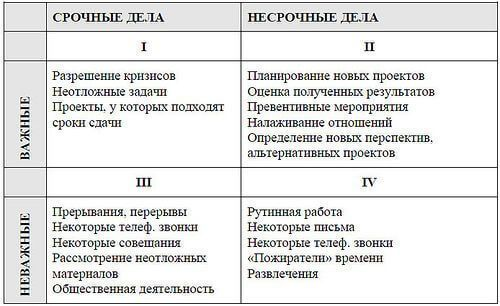
\includegraphics[scale=0.85]{images/eizinhower.jpg}  
  \caption{ Матрица Эйзенхауэра }
  \label{fig:domain:eizenhower}
\end{figure}

Организаторские способности Эйзенхауэра ценились всегда и везде. И совершенно заслуженно. Сейчас же матрицу Эйзенхауэра считают одним из самых эффективных средств для составления планов на короткий срок.



\subsubsection{Квадрант A: важные и срочные дела }


При идеальном планировании этот квадрант матрицы должен оставаться пустым, т.к. появление важных и срочных дел является показателем неорганизованности и допущения завала. Эта часть графика заполняется у многих людей из-за присущей им лени и неправильной расстановки приоритетов. Естественно, временами подобные дела могут появляться у каждого человека, но если это происходит ежедневно, то самое время обратить внимание на самодисциплину.

Итак, появления дел в квадранте A следует избегать. А для этого необходимо лишь вовремя выполнять пункты остальных квадрантов. Но если в первый квадрант что-то всё же и стоит вписывать, то это:

    Дела, невыполнение которых отрицательно сказывается на достижении поставленных целей
    Дела, невыполнение которых может стать причиной затруднений и неприятностей
    Дела, которые имеют отношение к здоровью

Важно также помнить о том, что существует такое понятие как «делегирование». Это означает, что при появлении в вашем квадранте A дел, которые можно кому-либо перепоручить, этой возможностью следует непременно воспользоваться для того чтобы как можно быстрее урегулировать другие важные и срочные дела.

\subsubsection{Квадрант B: важные, но не срочные дела }


Второй квадрант заслуживает наибольшего внимания, т.к. дела, находящиеся именно в нём, являются наиболее приоритетными и перспективными, и именно из них должны состоять повседневные задачи любого человека. Замечено, что люди, которые занимаются преимущественно делами этого квадранта, достигают в жизни наибольших успехов, продвигаются по службе, зарабатывают больше денег, имеют достаточно свободного времени и живут счастливой и насыщенной жизнью.

Обратите внимание также и на то, что отсутствие срочности позволяет подходить к решению любых задач более обдуманно и конструктивно, а это в свою очередь позволяет человеку раскрывать свой потенциал в полной мере, самостоятельно продумывать все нюансы своей деятельности и управлять временными рамками своих дел. Но здесь, помимо всего прочего, нужно помнить, что дела, находящиеся в квадранте B, если их не выполнять своевременно, могут с лёгкостью попасть в квадрант A, став ещё более важными и требующими скорейшего выполнения.

Опытные специалисты по организации времени рекомендуют включать в квадрант B все текущие дела, связанные с основной деятельностью, планирование и анализ работы, учебные и спортивные занятия, соблюдение оптимального графика и режима питания. Т.е. всё то, из чего состоит наша обычная повседневность.

\subsubsection{Квадрант C: срочные, но не важные дела }


Дела, которые находятся в этом квадранте, по большей части являются отвлекающими и нисколько не приближающими человека к намеченным результатам. Нередко они просто мешают сосредоточению на действительно важных задачах и снижают эффективность. Главное при работе с матрицей – не перепутать срочные дела из квадранта C со срочными делами из квадранта A. Иначе образуется неразбериха и то, что должно быть выполнено в первую очередь, остаётся на втором плане. Всегда помните о своих целях и учитесь отличать важное от второстепенного.

К делам квадранта C можно отнести, к примеру, навязанные кем-либо со стороны встречи или переговоры, празднования дней рождения не очень близких людей, внезапно возникшие хлопоты по дому, устранение не жизненно важных, но требующих внимания отвлекающих факторов (разбилась ваза, сломалась микроволновая печь, перегорела лампочка и т.п.), а также другие всевозможные дела, которые не продвигают вас вперёд, а только тормозят.

\subsubsection{Квадрант D: не срочные и не важные дела }


Задачи, относящиеся к последнему квадранту, не приносят совсем никакой пользы. Во многих случаях полезно не только заниматься ими в последнюю очередь, но и не заниматься ими вообще. Хотя знать о них непременно нужно, т.к. именно они являются «пожирателями времени».

Интересна и ещё одна особенность дел из данной группы: они являются очень привлекательными для многих людей – эти дела просты в выполнении и доставляют удовольствие, позволяют расслабиться и приятно провести время. Поэтому и противостоять соблазну ими позаниматься бывает довольно проблематично. Но делать это непременно нужно.

В квадрант D можно записать такие дела как разговоры по телефону с друзьями о чём-то несущественном, ненужная переписка или времяпрепровождение в соцсетях, просмотр сериалов и различных «отупляющих» телепередач, компьютерные игры и т.п. Конечно, отдыхать и как-то развлекать себя периодически должен каждый человек, но для этого существуют и более интересные и развивающие способы: чтение хороших книг, интеллектуальные игры, посещение спортзалов и бассейнов, поездки на природу и т.п. Если же полностью избавить себя от занятия делами из квадранта D не удаётся или не хочется, то нужно отложить их выполнение хотя бы до того момента, когда дела из квадрантов B и C будут выполнены, а время, которое будет уделяться делам квадранта D, должно быть сведено к минимуму.

\subsection{ Getting Things Done }

GTD, Getting Things Done — это система для самоорганизации, придуманная американским автором Дэвидом Алленом. С момента выпуска соответствующей книги в 2000 году миллионы неорганизованных людей наконец обрели счастье и душевное спокойствие. Ведь система, как заявляется, позволяет привети дела в порядок.

Основные принципы GTD очень просты. В основе лежат три привычки, к которым должен приучить себя каждый эффективный человек.
\begin{itemize}
  \item Записывать свои дела (Collect).
  \item Быстро решать, что делать дальше (Process).
  \item Делать то, что записал (Do).
\end{itemize}


\subsubsection{Collect. }

Почему многие люди испытывают постоянный стресс и ничего не успевают? Потому, что они хранят все дела в голове. А мозг человека способен одновременно удерживать в памяти только 7 объектов. Если хранить в голове слишком много мусора, многие вещи просто забываются и вспоминаются только тогда, когда уже поздно. В итоге получаются все эти «Забыл», «Не успел», «Ай, сделаю завтра»…

Первым шагом на пути к светлой голове будет отложить на 10 минут все дела в сторону, взять листок бумаги и выписать все дела, вопросы, идеи и прочие вещи, которые не дают вам покоя. Тем самым мы освобождаем голову и переносим все свои дела на «внешний носитель».
Пример? Пожалуйста. Слушаю я радио, и вдруг слышу рекламу про наступающий праздник 8 марта. В голову сразу приходит мысль «Не мешало бы купить подарок маме». Не откладывая в долгий ящик, сразу записываю: «Купить подарок маме на восьмое марта».
Готово? Переходим к следующему пункту.

\subsubsection{Process. }

На этом этапе нужно пройтись по всем записанным делам и для каждого из них задать себе один важный вопрос: какой следующий шаг?
Этот простой вопрос не так прост, как кажется. Например: вам нужно купить подарок маме и вы прилежно записали в блокнот «купить подарок маме на восьмое марта».
Что из этого получится? Скорее всего, вы будете долго искать себе отмазки, а подарок будет куплен в последний день. Ну и в результате накануне придется отстоять полдня в очередях, хотя на неделю раньше могли бы купить за пять минут.

Что в этом случае советует GTD.
GTD говорит вот что: сначала нужно выделить конкретный следующий шаг для покупки подарка. Конкретный шаг означает то, что ты оторвешься от стула и реально что-нибудь сделаешь. Например «Позвонить тете Ане и посоветоваться насчет подарка». Задача вдруг стала намного конкретнее, не правда ли? Теперь не нужно долго раздумывать: надо взять телефон и позвонить прямо сейчас.
Вот мы и пришли к третьему пункту.

\subsubsection{Do. }

Если до этого было сделалано всё правильно, то на данном этапе есть простая и понятная задача: «Позвонить тете Ане».
Так получается потому, что конечным итогом применения системы GTD является «кристально чистый» список «следующих шагов» по всем задачам. В этом списке собраны конкретные и понятные дела, которые можно выполнять без раздумий. Все раздумия уже проведены на этапе «Что дальше»?..

Теперь, при наличии такого кристально чистого списка, можно спокойно и не отвлекаясь щелкать дела одно за одним, как семечки. Никаких лишних терзаний, никаких сомнений — сплошной концентрированный поток действия. 

\section{Обзор аналогичных систем} 
\label{sec:practice:analogs}

\subsection{Doit.im}
\label{sub:practice:analogs:doit}
Мультиплатформенный  сервис для учета времени, имеет клиенты на Windows, OSX, Android, IOs а также веб версию. Как и любой другой сервис учет времени позволяет создавать задачи, и группы этих задач.

Отличительные черты данного проекта:

\begin{itemize}
  \item возможность добавллять к задачам контекс (прим. Работа, Быт и.др).
  \item возможность добавлять задаче тэги, и группировать по ним.
  \item возмжность создания задачи задавая параметры (контекст, тэг, проект и т.д.) с помощью специальных символов. Например, если ввести: Забрать сына из школы \string^Today @Семья \#Быт !High \&Дети –  будет создана задача “Забрать сына из школы” с датой выполнения Сегодня, имеющая контекст Семья, помещенная в проект Быт, с высоким приоритетом и которой будет присвоен тэг Дети.
\end{itemize}

\begin{figure}[ht]
\centering
  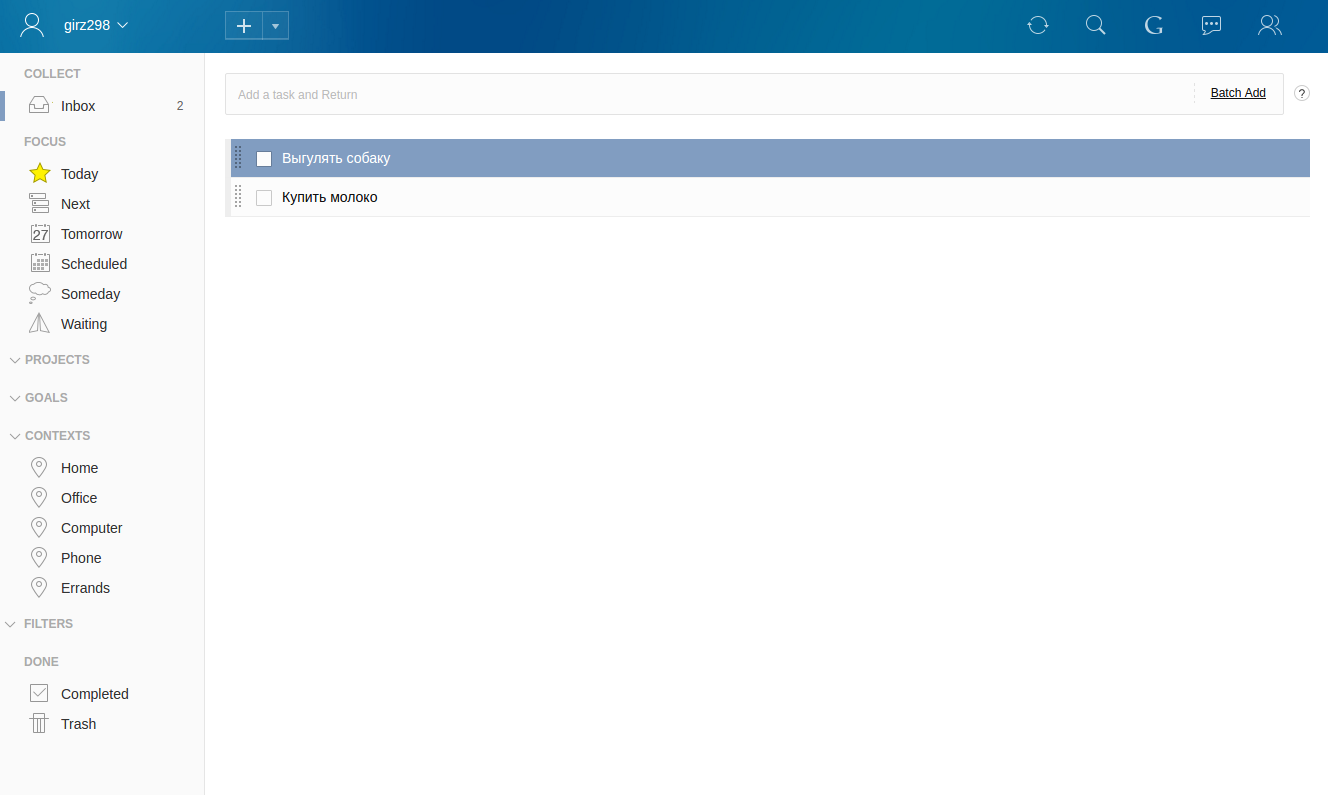
\includegraphics[scale=0.35]{images/doit.png}  
  \caption{ Основная страница веб-версии сервиса Doit.im }
  \label{fig:domain:doit.im}
\end{figure}

Doit.im — бесплатное приложение, однако ряд функций доступен только в PRO-версии. В любом случае бесплатно предоставляется 30-ти дневная бесплатная версия. Годовая подписка обойдется в \string$20. Еще один минус — отсутствие поддержки русского языка, кириллицу приложение распознает, но меню отображается только на английском. 

\subsection{Microsoft To-Do}
\label{sub:practice:analogs:microsoft_to_do}
Microsoft To-Do — это сервис для составления списка дел на день и распределения их по категориям. Функция «Интеллектуальные предложения» предложит оптимальный вариант распределения задач на основе прошлых записей. To-Do умеет импортировать задачи из Todoist и Wunderlist и синхронизироваться с приложениями из пакета Office. Доступно добавление заметок, напоминаний, повторов задач.

\label{page:domain:microsoft_to_do}
\begin{figure}[ht]
\centering
  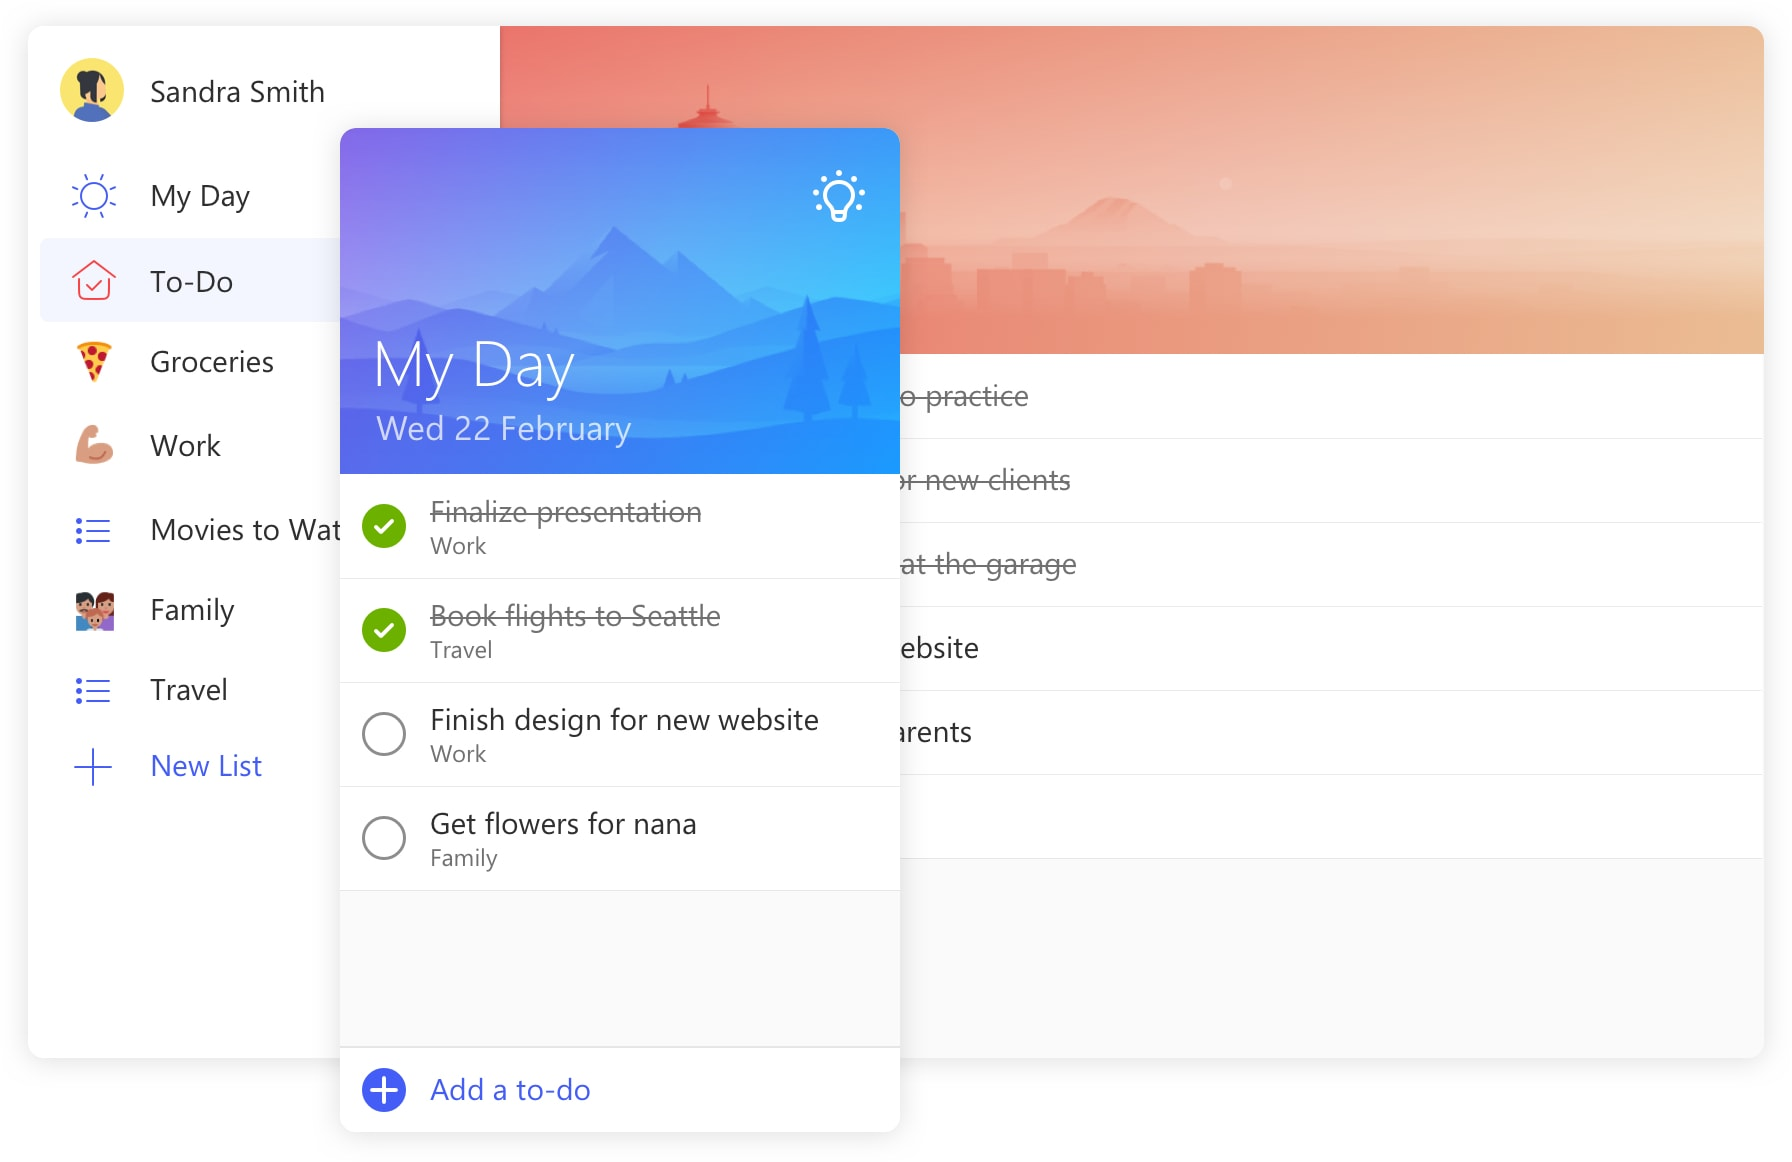
\includegraphics[scale=0.25]{images/microsoft_to_do.jpg}  
  \caption{ Мобильная и настольная версия Microsoft To-Do }
  \label{fig:domain:microsoft_to_do}
\end{figure}

\subsection{Remember the milk}
\label{sub:practice:analogs:remember_the_milk}

Этот сервис управления задачами считается одним из наиболее функциональных. Авторы Remember the Milk использовали принципы популярной техники управления задачами GTD, что и привело к появлению столь широкого набора функций. На первый взгляд количество параметров для задач в этом сервисе кажется слишком большим, и те пользователи, которым нужен просто список, наверняка не будут играться с заполнением всех этих полей. Для задачи в Remember the Milk можно указать срок выполнения, настроить повтор, задать ее продолжительность, добавить теги, место, ссылку, текстовые заметки, приоритет. Список мест формируется в специальном разделе и помогает напомнить, например, купить продукты в супермаркете, выполнить рабочие задачи в офисе и не забыть о домашней рутине, когда человек оказался дома. 

\begin{figure}[ht]
\centering
  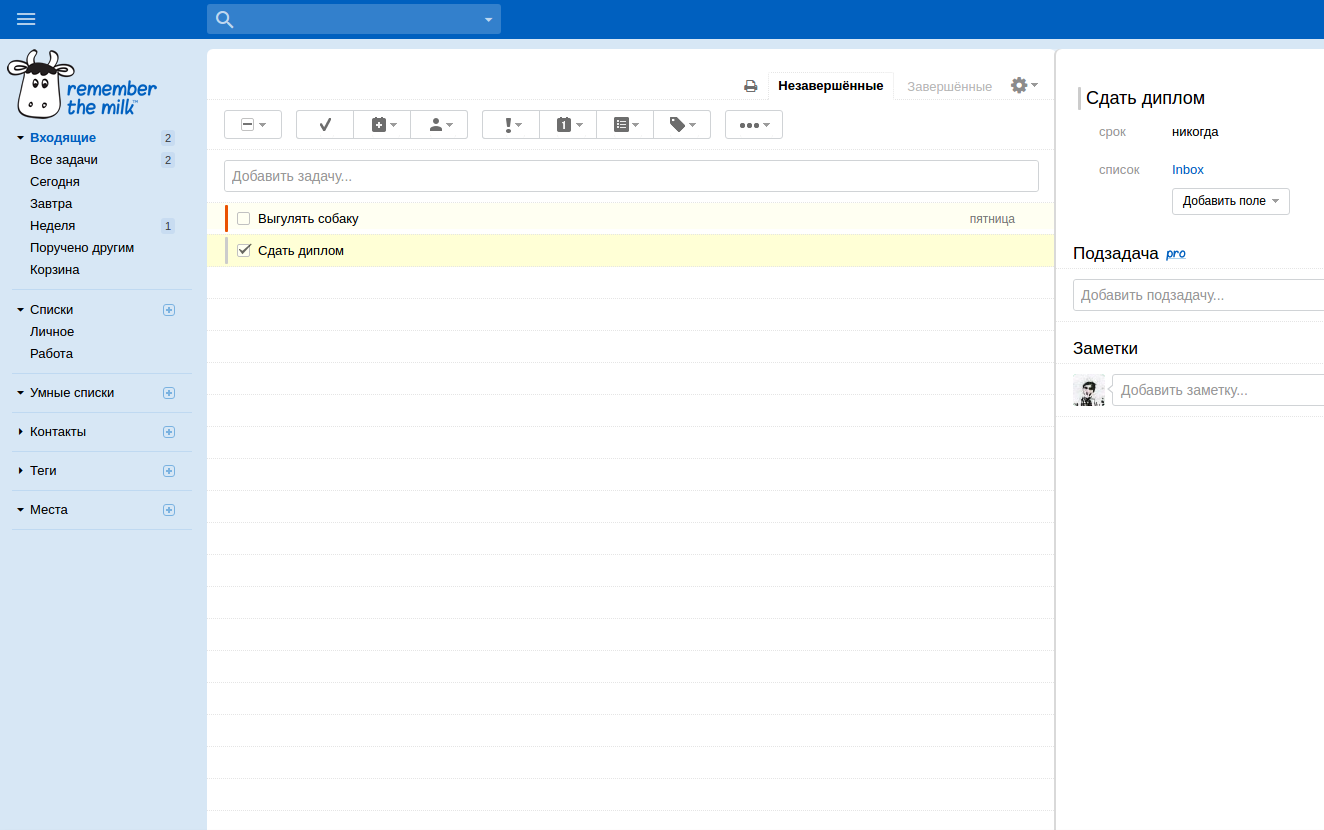
\includegraphics[scale=0.35]{images/remember_the_milk.png}  
  \caption{  Основная страница веб-версии сервиса Remember The Milk }
  \label{fig:domain:remember_the_milk}
\end{figure}

Отличительные черты данного проекта:

\begin{itemize}
  \item "умные" списки. Группируют задачи по спискам, классифицируя их по ключевым словам, заданным в описании этого списка.
  \item работа с геолокацией. 
  \item список контактов.
  \item возможность давать задачи пользователям из списка контактов.
\end{itemize}

В отличии от сервиса Doit.im в него добавлена полная поддержа русского языка, а также неплохой вводный курс на русском языке. Однако бесплатная версия ограничивается малой долей функционала. За полноценную PRO-версию без ограничений функционала авторы просят \string$40 в год.

\subsection{Todoist}
\label{sub:practice:analogs:todoist}

Кроссплатформенный проект с многомилионной аудиторией. Имеет интеграцию с многими сервисами, облачную синхронизацию, интуитивно понятный интерфейс и полную русскую локализацию. Для работы нужно создать новый проект(группу задач), затем добавить в него задачи, указав их описание и планируемые сроки выполнения.  Приоретизация задач основана на матрице Эйзенхауэра. 

Отличительные черты данного проекта:

\begin{itemize}
  \item есть возможность создание команды(группы пользователей) и командного выполнения задач.
  \item приоритизация задач основана на матрице Эйзенхауэра. 
  \item отличная кроссплатформенная поддержка от Apple Watch до Symbian устройств.
\end{itemize}


\begin{figure}[ht]
\centering
  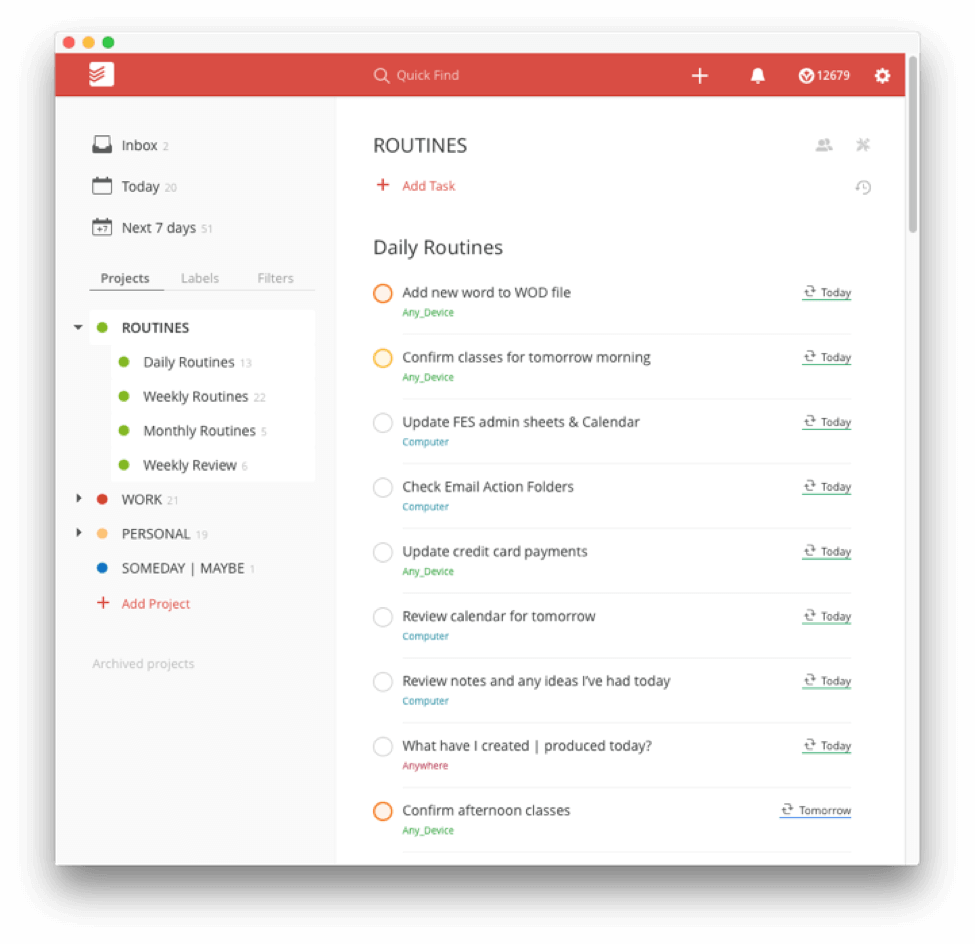
\includegraphics[scale=0.42]{images/todoist.png}  
  \caption{  Основная страница веб-версии сервиса Todoist }
  \label{fig:domain:todist}
\end{figure}

Также как и в аналогичных сервсах у этого есть PRO-версия стоимостью \string$29 в год. Пользователи с PRO-версией могут добавлять комментарии к своим задачам, просматривать завершённые задачи, отправлять задачи по электронной почте, получать напоминания на почту или через SMS, экспортировать задачи в календарь Google, Outlook или iCal, использовать поиск и просматривать статистику своей продуктивности по дням и проектам.

\section{Используемые технологии} 
\label{sec:practice:technology_used}
Выбор технологий является важным предварительным этапом разработки сложных информационных систем. Платформа и язык программирования, на котором будет реализована система, заслуживает большого внимания, так как исследования показали, что выбор языка программирования влияет на производительность труда программистов и качество создаваемого ими кода ~\cite{mcconnell_2005}.

Ниже перечислены некоторые факторы, повлиявшие на выбор технологий:
\begin{itemize}
  \item Среди различных языков программирования разработчик имеет наибольший опыть в PHP.
  \item Разработчик имеет опыт работы с объектно-ориентированными языками программирования, и решениями в полной мере реализующие возможности ООП.
  \item Платформа Symfony хорошо подходит для реализации серверной бизнес - логики приложения, и разработчик имеет опыт работы с этой платформой.
\end{itemize}


\subsection{Язык программирования PHP}
\label{sub:practice:php_overview}
PHP (Hypertext Preprocessor - «PHP: препроцессор гипертекста»; первоначально Personal Home Page Tools - «Инструменты для создания персональных веб-страниц») - скриптовый язык общего назначения, интенсивно применяемый для разработки веб-приложений. В настоящее время поддерживается подавляющим большинством хостинг-провайдеров и является одним из лидеров среди языков, применяющихся для создания динамических веб-сайтов~\cite{php_documents}.

Главная область применения PHP - написание скриптов, работающих на стороне сервера; таким образом, PHP способен выполнять все то, что выполняет любая другая программа CGI, например, обрабатывать данные форм, генерировать динамические страницы или отсылать и принимать cookies. Но PHP способен выполнять намного больше.

PHP доступен для большинства операционных систем, включая Linux, многие модификации Unix (такие как HP-UX, Solaris и OpenBSD), Microsoft Windows, Mac OS X, RISC OS, и многие другие. Также в PHP включена поддержка большинства современных веб-серверов, таких как Apache, IIS и многих других. Подойдет любой веб-сервер, способный использовать бинарный файл FastCGI PHP, например, lighttpd или nginx. PHP может работать в качестве модуля или функционировать в качестве процессора CGI.

Таким образом, выбирая PHP, вы получаете свободу выбора операционной системы и веб-сервера. Более того, у вас появляется выбор между использованием процедурного или объектно-ориентированного программирования (ООП) или же их сочетания.

PHP способен генерировать не только HTML. Доступно формирование изображений, файлов PDF и даже роликов Flash (с использованием libswf и Ming), создаваемых «на лету». PHP также способен генерировать любые текстовые данные, такие, как XHTML и другие XML-файлы. PHP может осуществлять автоматическую генерацию таких файлов и сохранять их в файловой системе вашего сервера вместо того, чтобы отдавать клиенту, организуя, таким образом, серверный кэш для вашего динамического контента.

Одно из преимуществ язка PHP - поддержка широкого круга баз данных. Для создания сценария использующего базу данных можно воспользоваться расширением, специфичным для отдельной базы данных (таким как mysql) или использовать уровень абстракции от базы данных, такой как PDO, или подсоединиться к любой базе данных, поддерживающей Открытый Стандарт Соединения Баз Данных (ODBC), с помощью одноименного расширения ODBC. Для других баз данных, таких как CouchDB, можно воспользоваться cURL или сокетами~\cite{php_documents}.

PHP также поддерживает «общение» с другими сервисами через такие протоколы, как LDAP, IMAP, SNMP, NNTP, POP3, HTTP, COM (на платформах Windows) и многих других. Кроме того, вы получаете возможность работать с сетевыми сокетами напрямую. PHP поддерживает стандарт обмена сложными структурами данных WDDX практически между всеми языками веб-программирования. Обращая внимание на взаимодействие между различными языками, следует упомянуть о поддержке объектов Java и возможности их использования в качестве объектов PHP.

PHP имеет много возможностей по обработке текста, включая регулярные выражения Perl (PCRE) и много других расширений и инструментов для обработки и доступа к XML документам. В PHP обработка XML-документов стандартизирована и происходит на базе мощной библиотеки lib-xml2, расширив возможности обработки XML добавлением новых расширений SimpleXML, XMLReader и XMLWriter~\cite{php_documents}.

\subsubsection{Область применения. }
\label{sub:practice:whereis_php}
В области веб-программирования, в частности серверной части, PHP - один из популярных сценарных языков (наряду с JSP, Perl и языками, используемыми в ASP.NET).

Популярность в области построения веб-сайтов определяется наличием большого набора встроенных средств для разработки веб-приложений. 

Основные из них:
\begin{itemize}
  \item автоматическое извлечение POST и GET-параметров, а также переменных окружения веб-сервера в предопределённые массивы;
  \item взаимодействие с большим количеством различных систем управления базами данных, такми как: MySQL,  SQLite, PostgreSQL, Oracle, ODBC и др
  \item автоматизированная отправка HTTP-заголовков;
  \item работа с HTTP-авторизацией;
  \item работа с локальными и удалёнными файлами, сокетами;
  \item обработка файлов, загружаемых на сервер;
  \item работа с cookies и сессиями;
\end{itemize}

В настоящее время PHP используется сотнями тысяч разработчиков. Согласно рейтингу корпорации TIOBE, базирующемся на данных поисковых систем, в мае 2016 года PHP находился на 6 месте среди языков программирования. К крупнейшим сайтам, использующим PHP, относятся Facebook, Wikipedia, Vkonakte, Badoo и др.



\subsubsection{Элементарные типы PHP. }
\label{sub:practice:types_php}

РНР является слабо типизированным языком. Это означает, что нет необходимости объявлять тип данных, который должна хранить переменная. Так, в пределах одной и той же области видимости переменная \$number может содержать как значение 2, так и строку " two " ("два"). В строго типизированных языках программирования, таких как С или Java, вы обязаны определить тип переменной , прежде чем присваивать ей значение, и, конечно, это значение должно быть указанного типа. Но это не означает, что в РНР нет понятия типа. Каждое значение, которое можно присвоить переменной, имеет свой тип~\cite{zandstra_2015}.

Ниже представлены элементарные типы языка PHP:
\begin{itemize}
  \item Boolean - одно из двух значений true или false;
  \item Integer - целое число;
  \item Double - число с плавающей точкой;
  \item String - символьные данные(строка);
  \item Array - массив;
  \item Object - объект;
  \item Resource - дескриптор, используемый для идентификации и работы с внешними ресурсами , такими как базы данных или файлы; 
  \item Null - неинициализированное значение;
\end{itemize}


\subsubsection{Объектно-ориентированное программирование. }
\label{sub:practice:oop_php}
Ключевое слово class было зарезервировано ещё в третьей версии языка. В четвёртой версии стало возможно создавать классы и объекты на их основе. Однако принципы ООП поддерживались лишь частично, так например, все члены (переменные и методы) были открыты. К тому же создание объектов было дорогой операцией и работали они медленно.

Начиная с пятой версии PHP обладает полной поддержкой ООП. Работа с классами была оптимизирована и теперь такой код работает достаточно быстро.

Класс в PHP объявляется с помощью ключевого слова class. Методы и поля класса могут быть общедоступными (public, по умолчанию), защищёнными (protected) и скрытыми (private). PHP поддерживает все три основных механизма ООП - инкапсуляцию, полиморфизм подтипов и наследование (родительский класс указывается с помощью ключевого слова extends после имени класса). Поддерживаются интерфейсы (ставятся в соответствие с помощью implements). Разрешается объявление финальных, абстрактных методов и классов. Множественное наследование классов не поддерживается, однако класс может реализовывать несколько интерфейсов. Для обращения к методам родительского класса используется ключевое слово parent.

Начиная с версии 5.4.0 множественное наследование может быть реализовано с помощью механизма трейтов. Повторное использование кода заключено в использовании кода трейта в нескольких классах. Допускается использовать в одном классе несколько трейтов. Механизм трейтов имеет средства разрешения конфликтов имён. При запуске программы код трейта будет «вкомпилирован» в код содержащего его класса.

Классы в PHP имеют ряд «магических» методов, начинающихся с двух символов подчёркивания. Особо стоит отметить конструктор (\_\_construct(), в версиях до 5.0 конструктором служил метод, одноимённый с классом) и деструктор (\_\_destruct()), а также методы чтения (\_\_get()) и записи (\_\_set()), свёртывания (\_\_sleep()) и развёртывания (\_\_wakeup()), клонирования (\_\_clone()) и др. Эти методы являются достаточно гибким инструментом: переопределяя их, можно добиться существенного изменения поведения объекта.

Экземпляры класса создаются с помощью ключевого слова new, обращение к полям и методам объекта производится с использованием оператора "->", для доступа к метода и свойствам объявленным с ключевым словом static используется оператор "::". Для доступа к членам класса из его методов используется переменная \$this.

Пример объектно-ориентированной конструкции на языке PHP: 
\begin{lstlisting}
          class C1 extends C2 implements I1, I2
          {
            private $a;
            protected $b;

            function __construct($a, $b)
            {
              parent::__construct($a, $b);
              $this->a = $a;
              $this->b = $b;
            }

            public function plus()
            {
              return $this->a + $this->b;
            }
          }

          $d = new C1(1, 2);
          echo $d->plus(); // 3
\end{lstlisting}

\subsubsection{Объектно-ориентированное программирование. }
\label{sub:practice:extebtions_php}
Интерпретатор состоит из ядра и подключаемых модулей, «расширений», представляющих собой динамические библиотеки. Расширения позволяют дополнить базовые возможности языка, предоставляя возможности для работы с базами данных, сокетами, динамической графикой, криптографическими библиотеками, документами формата PDF и тому подобным. Любой желающий может разработать своё собственное расширение и подключить его. Существует огромное количество расширений, как стандартных, так и созданных сторонними компаниями и энтузиастами, однако в стандартную поставку входит лишь несколько десятков хорошо зарекомендовавших себя. Множество расширений доступно в репозитории PECL.

Ниже представлены «расширения» языка использованные в этой дипломной работе:
\begin{itemize}
  \item mbstring - предоставляет функции для работы с многобайтными строками, которые облегчают работу c многобайтными кодировками в PHP. Кроме того, mbstring занимается конвертированием строк из одной кодировки в другую. mbstring предназначен для работы с Unicode-кодировками, такими, как UTF-8 и UCS-2, а также с многими однобайтными кодировками;
  \item xml - Данное расширение позволит вам создавать XML - анализаторы и далее определить обработчики для различных событий. Каждый XML-анализатор также имеет несколько параметров, которые вы можете настраивать. В работе требовалось для корректной работы с YAML файлами конфигураций платформы Symfony;
  \item pdo - определяет простой и согласованный интерфейс для доступа к базам данных в PHP;
\end{itemize}

\subsubsection{Режимы запуска интерпретатора. }
\label{sub:practice:extebtions_php}

SAPI - это внешний уровень абстракции, предназначенный для встраивания интерпретатора в другие приложения и отвечает за его работу (запуск, остановка, передача скриптов на исполнение, доступ к внешним данным). Существует несколько основных SAPI определяющих способы запуска и использования PHP:

\begin{itemize}
    \item   В качестве модуля к веб-серверу (прим. Apache модуль mod\_php). В этом случае интерпретатор PHP выполняется в окружении процесса веб-сервера. Веб-сервер управляет количеством запущенных процессов PHP и сообщает им какие скрипты требуется исполнить.

    \item   CGI SAPI. Использование CGI подразумевает запуск нового процесса для обработки каждого запроса. Для исполнения PHP скрипта веб-сервер запускает ./php-cgi /path/to/script.php. Сам принцип такого использования подразумевает, что интерпретатор PHP исполняет только один скрипт, после чего заканчивает свою работу. Затраты на запуск процесса интерпретатора и его инициализацию очень часто сопоставимы или даже превышают затраты на исполнение PHP скрипта. Для решения этой проблемы в CGI SAPI был введен режим FastCGI. В этом режиме PHP интерпретатор запускается как независимый сервер, обрабатывающий входящие запросы на исполнение PHP скриптов по протоколу FastCGI, что позволяет ему работать с любым веб-сервером поддерживающим этот протокол~\cite{php_documents}.

    \item   FPM SAPI, известный как php-fpm - это другая реализация протокола FastCGI. Создан изначально Андреем Нигматулиным как отдельный патч для использования в социальной сети Badoo. Данная реализация решала ряд проблем, которые мешали использованию CGI/FastCGI SAPI. В частности, появилась возможность перезапуска пула интерпретаторов PHP без потери запросов, запуск нескольких пулов под разными пользователями, аварийный перезапуск интерпретаторов в случае проблем с ними и ещё несколько приятных дополнений. В дальнейшем над патчем работали несколько человек, был добавлен режим динамического управления числом запущенных процессов PHP (по принципу управления числом процессов в веб-сервере Apache), и начиная с версии PHP 5.3.3 php-fpm был включен в PHP как отдельное SAPI.

    \item   В качестве скрипта командной строки (CLI SAPI), являющегося исполняемым файлом, который вызывается пользователем из командной строки; скрипт выполняется в окружении вызвавшего пользователя. В этом случае возможно использование PHP для создания клиентских GUI-приложений и решения административных задач в операционных системах UNIX, Linux, Microsoft Windows, Mac OS X и AmigaOS. Однако в таком качестве он не получил распространение, отдавая первенства Perl, Python и VBScript.
    Начиная с версии PHP 5.4.0 в CLI SAPI появилась возможность запуска PHP как отдельного HTTP сервера. Однако этот режим предназначен исключительно для разработки, так как запускает только один процесс интерпретатора и выполняет все запросы исключительно последовательно~\cite{php_documents}.
\end{itemize}


\subsection{Платформа Symfony}
\label{sub:practice:symfony}

Symfony - свободная программная платформа, написанная на PHP, который использует паттерн Model-View-Controller.

Symfony предлагает быструю разработку и управление веб-приложениями, позволяет легко решать рутинные задачи веб-программиста. Работает только с PHP 5 и выше. Имеет поддержку множества баз данных (MySQL, PostgreSQL, SQLite или любая другая PDO-совместимая СУБД). Информация о реляционной базе данных в проекте должна быть связана с объектной моделью. Это можно сделать при помощи ORM инструмента. В Symfony это Doctrine.

Symfony бесплатен и публикуется под лицензией MIT.

\subsection{ORM Doctrine}
\label{sub:practice:doctrine}
Doctrine - объектно-реляционный проектор (ORM) для PHP 5, который базируется на слое абстракции доступа к БД (DBAL). Одной из ключевых возможностей Doctrine является запись запросов к БД на собственном объектно-ориентированном диалекте SQL, называемый DQL (Doctrine Query Language) и базирующийся на идеях HQL (Hibernate Query Language).

Doctrine cледует паттерну Data mapper. Для создания пользователя может использоватся следующий код:

\begin{lstlisting}
          $user = new User();
          $user->setName("john");
          $user->setPassword("doe");
          $entityManager->persist($user);
          $entityManager->flush();
          echo "The user with id " . $user->getId() . "has been saved.";
\end{lstlisting}


Получение оъекта класса Product соответствующего строке в базе данных по уникальному \$id:
\begin{lstlisting}
          $em = $this->getDoctrine();
          $product = $em->getRepository('AcmeStoreBundle:Product')->find($id);
\end{lstlisting}

Добавление оъекта класса Product с именем 'Name' в базу данных:
\begin{lstlisting}
          $product = new Product();
          $product->setName('Name');
          $em = $this->getDoctrine()->getManager();
          $em->persist($product);
          $em->flush();
\end{lstlisting}

Одной из особенностей Doctrine является низкий уровень конфигурации, необходимый для запуска проекта. Doctrine может генерировать классы объектов из существующей базы данных, и программист может затем указать отношения и добавить пользовательские функциональные возможности к сгенерированным классам. Нет необходимости создавать или поддерживать сложные схемы базы данных XML, как это видно во многих других платформах.

Еще одной важной особенностью Doctrine является возможность произвольной записи запросов базы данных в диалекте OO (объектно - ориентированный) SQL, называемом DQL (Doctrine Query Language), который был разработан на основе  HQL Hibernate. Класс QueryBuilder позволяет создавать запросы через свободный интерфесы. Эти интерфейсы предоставляют разработчикам мощные альтернативы SQL, которые поддерживают гибкость и позволяют переключать базы данных, не требуя дублирования кода.

Ниже представлен пример испольования QueryBuilder в Doctrine:
\begin{lstlisting}
          $repository = $this->getDoctrine()->getRepository('AppBundle::Product');
          $query = $repository
                      ->createQueryBuilder('p')
                      ->where('p.price>:price')
                      ->setParameter('price','19.99')
                      ->orderBy('p.price','ASC')
                      ->getQuery();
          $products = $query->getResult();
\end{lstlisting}

Явное написание запросов к БД не всегда необходимо, так как Doctrine выполняет объединения и выбирает связанные объекты автоматически. Малые проекты можно построить не используя запросы.

\section{Проектирования системы организации времени}

Перед разработкой любой системы к ней предъявляется ряд требовний, таких как функционал, который должна предоставлять система, сроки разработки, покрытие системы автоматизированными тестами и возможность расширения системы. Следовательно проектирование можно сформулировать как поиск оптимального решения для удовлетворения всех требований представленных данной системе.

Одним из инструментов проектирования программного обеспечения является унифицированный язык моделирования UML. UML — язык графического описания для объектного моделирования в области разработки программного обеспечения, системного проектирования и отображения организационных структур.

На этапе проектирования были выделены основные сущности системы, представленные ниже на диаграмме "сущность-связь".

\begin{figure}[ht]
\centering
  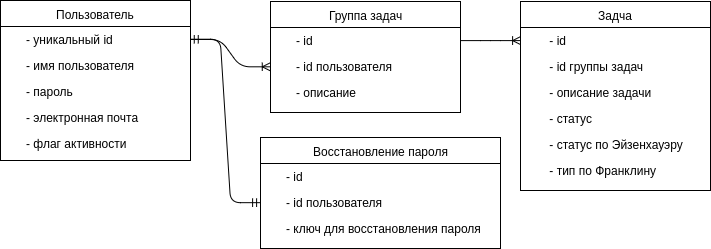
\includegraphics[scale=0.5]{images/entity-relation.png}  
  \caption{ Диаграмма сущность-связь для системы организации времени }
  \label{fig:domain:todist}
\end{figure}

Следом после построения диаграммы "сущность-связь", можно построить базы данных MySQL, определив типы полей.

\begin{figure}[ht]
\centering
  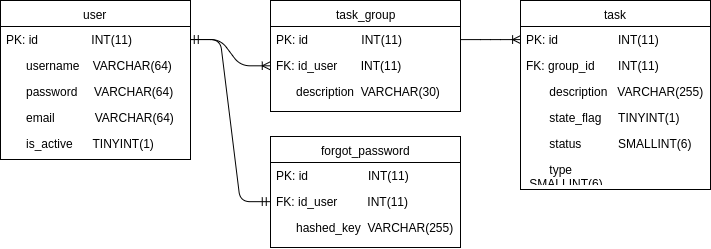
\includegraphics[scale=0.5]{images/mysql_schema.png}  
  \caption{ Схема базы даннных для системы организации времени }
  \label{fig:domain:todist}
\end{figure}

